
\title{Recap Database Management System (01NVVOV)}
\author{Jacopo Nasi\\
        Computer Engineer\\
        Politecnico di Torino}
\date{I Period - 2017/2018\\\bigskip\bigskip\today}

\documentclass[12pt]{article}
\usepackage[utf8]{inputenc}
\usepackage[italian]{babel}
\usepackage{geometry}
\usepackage{indentfirst} % First line indent
\usepackage{mathtools}
\usepackage{wrapfig}
\usepackage[usenames, dvipsnames]{color}
\usepackage{float}
\usepackage{amssymb}
\usepackage{ifsym}
% Misure Documento
\geometry{ a4paper, total={170mm,257mm},left=35mm, right=35mm, top=35mm, bottom=35mm }

\begin{document}

\begin{figure}
  \centering
  
\includegraphics[width=10cm]{images/polito.pdf}
\end{figure}

\maketitle

\newpage
\tableofcontents

\newpage
{\noindent \Large \textbf{License}\bigskip}

This work is licensed under a Creative Commons Attribution-NonCommercial-ShareAlike 3.0 Unported License.\\
You are free:
\begin{itemize}
  \item \textbf{to Share}: to copy, distribute and transmit the work
  \item \textbf{to Remix}: to adapt the work
\end{itemize}
Under the following conditions:
\begin{itemize}
  \item \textbf{Attribution}: you must attribute the work in the manner specified by the author or licensor (but not in any way that suggests that they endorse you or your use of the work)
  \item \textbf{Noncommercial}: you may not use this work for commercial purposes.
  \item \textbf{Share Alike}: if you alter, transform, or build upon this work, you may distribute the resulting work only under the same or similar license to this one.
\end{itemize}

\noindent More information on the Creative Commons website (http://creativecommons.org).

\begin{figure}[h!]
  \centering
  
\includegraphics[width=3cm]{images/license.png}
\end{figure}

{\noindent \Large \textbf{Acknowledgments}\bigskip}

Questo breve riepilogo non ha alcuno scopo se non quello di agevolare lo studio di me stesso, se vi fosse di aiuto siete liberi di usarlo.\\
Le fonti su cui mi sono basato sono quelle relative al corso offerto (\textbf{Database Management System (01NVVOV)}) dal Politecnico di Torino durante l'anno accademico 2017/2018.\\
Non mi assumo nessuna responsabilità in merito ad errori o qualsiasi altra cosa. Fatene buon uso!
\newpage

\section{Database Management System}
\subsection{Introduction}

The DataBase Management System \textbf{DBMS} is a software package designed to store and manage databases. The architecture of the system is similar to the one in the figure \ref{fig:arch}.
\begin{figure}[h!]
  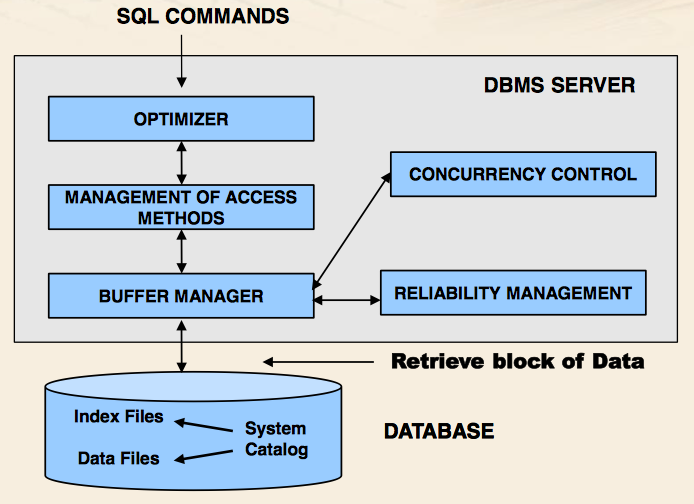
\includegraphics[width=\linewidth]{images/arch.png}
  \caption{DBMS Architecture}
  \label{fig:arch}
\end{figure}
Since the DB data part can be really big it can't fit always in the main memory (RAM) and, for this fact, is often stored in the secondary memory, like HDD. For this reason is necessary a system that define the operations to grab and manage the data from the secondary memory.\\
All the blocks has different behaviours. The \textbf{Optimizer} have multiple roles:
\begin{itemize}
  \item Define an appropriate execution strategy for accessing data to answer queries.
  \item Receives in input the SQL instructions (DML).
  \item Check the lexical, syntactical and sematical correctness (not all the errors).
  \item Translate the query in an internal algebra rappresentation.
  \item Select the "right" strategy for accesing data.
  \item Guarantees the \textbf{data independence} property in the relation model.
\end{itemize}
The \textbf{Access Method Manager} is used for physical access to data and it implements the strategy selected by the optimizer. The \textbf{Buffer Manager} instead manage the page transfert from disk to main memory and vice versa and the main memory portion that is pre-allocated to the DBMS that is shared among many applications. The \textbf{Concurrency Control} coordinate the concurrent access to data (important for write operations) to guarantess the consistency of it. The \textbf{Realiability Manager} guarantees correctness of the database content duing the system crashes, the atomic execution of a transaction and it exploits auxiliary structures (log files) the correct the database in case of failure.\\
The \textbf{transaction} is an unit of work performed by an application, it's a sequence of one or more SQL RW operation charaterized by \textit{correctness, reliability} and \textit{isolation}. The START of a transaction is typically implicit and coincides with the first SQL instruction. The END instead can be of two differents types, it can be a COMMIT that it means the correct end of a transaction, or with ROLLBACK that it means error during the execution. In this second case the DBMS needs to go back to the state at the beginning of the transaction. The rollback can be of two type suicide, when is required by the transaction, and murder when is required by the system. The transaction have four important properties:
\begin{itemize}
  \item \textbf{A}tomicity
  \item \textbf{C}onsistency
  \item \textbf{I}solation
  \item \textbf{D}urability
\end{itemize}
Atomicity means that they cannot be divided in smaller units, is not possibile to leave the system in a intermediate state of exec, guarantee by UNDO (undoes all the work perfomed, used for rollback) and REDO (redoes all work performed, used for commit the result in presence of failure). The consistency means that the transaction execution should not violate integrity constraints on a database, in case of it the system will perform solution to correct the violation. The system can be considered Isolated when the execution of a transaction is indipendent of the concurrent execution of other transaction, everything is enforced by the Concurrency Control block. The last properties means that, in presence of failures, the effect of a commited transaction IS NOT LOST, it guarantees the reliability of the DBMS and is enforced by the Reliability Manager block. % 3/9/17 @ 18:15

\subsection{Buffer Manager}
This block have a real important behaviour, it manages page transfer from disk to main memory and it's in charge of managing the DBMS buffer. The operation of the pages trasnfert is the bottleneck of every system and this is why this block is really important. increasing the performance of this operation could really improve the speed of the entire system.\\
The buffer is:
\begin{itemize}
  \item A large main memory block.
  \item Pre-allocated to the DBMS.
  \item Shared among executing transactions.
\end{itemize}
this part is organized in pages where the size depends on the size of the OS I/O block. There are two empirical law often used for hte management strategies:
\begin{enumerate}
  \item Data Locality: Data referenced recntly is likely to be referenced again.
  \item 20-80: The 20\% of data is RW by 80\% of transaction.
\end{enumerate}
The buffer manager keeps additional snapshot information on the current content of the buffer, it shot, for every page, the physical location of the page on the secondary memory (file identifier and block number) and two state variables, one that count of the number of trasn using the page in that time (count), and the dirty bit that is set if the page has been modified.\\ %Set No. 2 @ PAG. 8
It provides different access methods to load pages from disk and vice versa:
\paragraph{Fix Primitive} used by transactions to require access to a disk page, after the page is loaded into the buffer a pointer is returned to the requesting transaction and the Count is incremented by 1. This procedure requires an I/O operation only id the page is not already in the buffer. There are two behaviour:
\begin{itemize}
  \item Page already in buffer: Return the pointer to the data.
  \item Page not in buffer: It search a place for the page.
  \begin{enumerate}
    \item Free pages
    \item Not free pages, Count=0; if the data is dirty it performs a synchronous write on the disk.
  \end{enumerate}
\end{itemize}
\paragraph{Unfix Primitive} it tells the buffer manager that the transaction is no longer using the page and it decrease the Count.
\paragraph{Set Dirty Primitive} is tells the buffer manager that the page has been modified by the running transaction and it sets the dirty bit to 1.
\paragraph{Force Primitive} it requires a synchronous transfert of the page to the disk, when this operation is performed the transaction is suspended.
\paragraph{Flush Primitive} is an autonomous transfert of the pages on the disks, is internal to the buffer manager and is runned when the CPU is not too much loaded. It transfer the page that are not valid (count=0) or not accessed since long time.\\
The are four writing strategies:
\begin{itemize}
  \item \textbf{Steal}: The BM is allowed to select a locked page with Count=0 as victim. It writes on disk the dirty pages belonging to uncommitted trans. It can be undone.
  \item \textbf{No Steal}: The BM is not allow to steal.
  \item \textbf{Force}: All the pages are synchronous written on the disk during the commit operation.
  \item \textbf{No Force}: The pages are written asynchronously with the Flush Primitive.
\end{itemize}
The mostly used solution is \textbf{steal/no force} because of its efficency. The no force provides better I/O performance, steal may be mandatory for queries accessing a very large number of pages.

\paragraph{File System} the BM is using services provided by the file system:
\begin{itemize}
  \item Create/Delete of a file.
  \item Open/Close file.
  \item Read: It provides a direct access to a block in a file and it requires File Identifier, Block number and buffer page where to save data.
  \item Sequential Read: It provides seq. access to a fixed number of blocks in a file, it requires file identifier, strating block, number of blocks to be readed and the starting page for saving.
  \item Write and Sequential Write.
  \item Directory management.
\end{itemize} % END Block 2 - Buffer Manager

\subsection{Physical Access}
Data may be stored in different format to provide efficient query execution. The \textbf{Access Method Manager} transform the decision taken by the optimizer into sequence of physical access to data. An access method is a software module specialized for single data structure that provide primitives for read and write. The AM can select the appropriate blocks of a file to be loaded in memory and it knows the organization of data into a page.\\
There are several solution for manage the data in relational system:
\begin{itemize}
  \item Physical data storage
  \begin{itemize}
    \item Sequential Structure
    \item Hash Structure
  \end{itemize}
  \item Indexing
  \begin{itemize}
    \item Tree Structure
    \item Unclustered Hash Index
    \item Bitmap Index
  \end{itemize}
\end{itemize}

In the sequential solution the tuples are stored in a given sequential order, in the case of the heap file are sorted in the insertion order, typically append at the end of the file.
\begin{itemize}
  \item \textbf{PRO}: No wasted space, sequential read/write fast.
  \item \textbf{CONS}: Delete may cause wasted space.
\end{itemize}
this structure are frequently used jointly with unclustered indices to support search and sort operations.\\
In the ordered structures everything is sorted by the value of a given key, called sort key, it can contain one or more attributes.
\begin{itemize}
  \item \textbf{PRO}: Sort, group by, search or join operations on the sort key really fast.
  \item \textbf{CONS}: Inserting new value preserving order.
\end{itemize}
the main problem of this solution is to keep the order of the data during new data insertion. There are two main solution, the first il leaving a percentage of free space in each block during the table creation; the second one create an overflow file containing tuples which do not fit into the correct block.\\
The ordered structure are typically used with $B^{+}$-Tree clustered (primary) indices where the index key is the sort key. Are used bt the DBMS too to storing intermediate operation results. This structure provide "direct" access to data based on a key (one or more attributes). This Tree have one root node with many intermediate nodes and each node has many children. The leaf nodes provide access to data in 2 different ways:
\begin{itemize}
  \item \textbf{Clustered}: It store the data in the main memory. Used for primary key indexing. [figure \ref{fig:clu}]
  \item \textbf{Unclustered}: It store a pointer to the secondary memory of the data. Used for secondary indices. [figure \ref{fig:unclu}]
\end{itemize}
\begin{figure}[!hbpt]
  \centering
  \begin{minipage}{.45\textwidth}
    \centering
    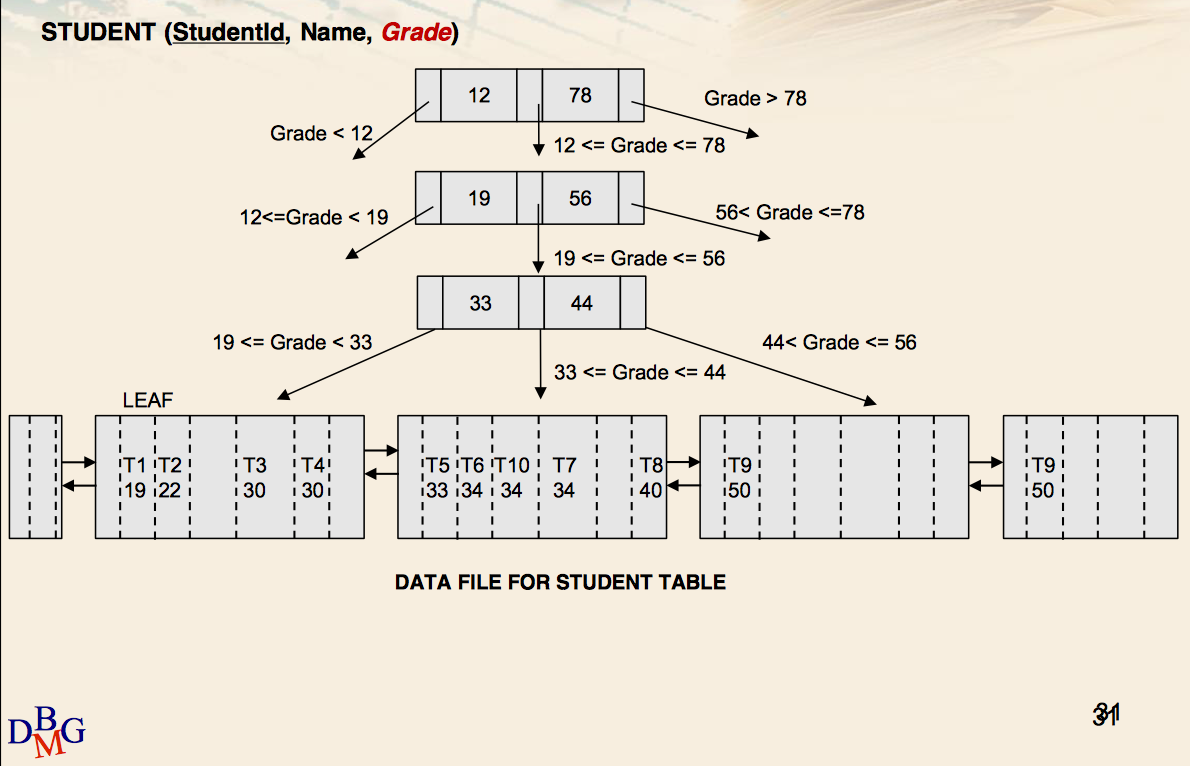
\includegraphics[width=\linewidth]{images/clu.png}
    \caption{Clustered}
    \label{fig:clu}
  \end{minipage}\hfill
  \begin{minipage}{.45\textwidth}
    \centering
    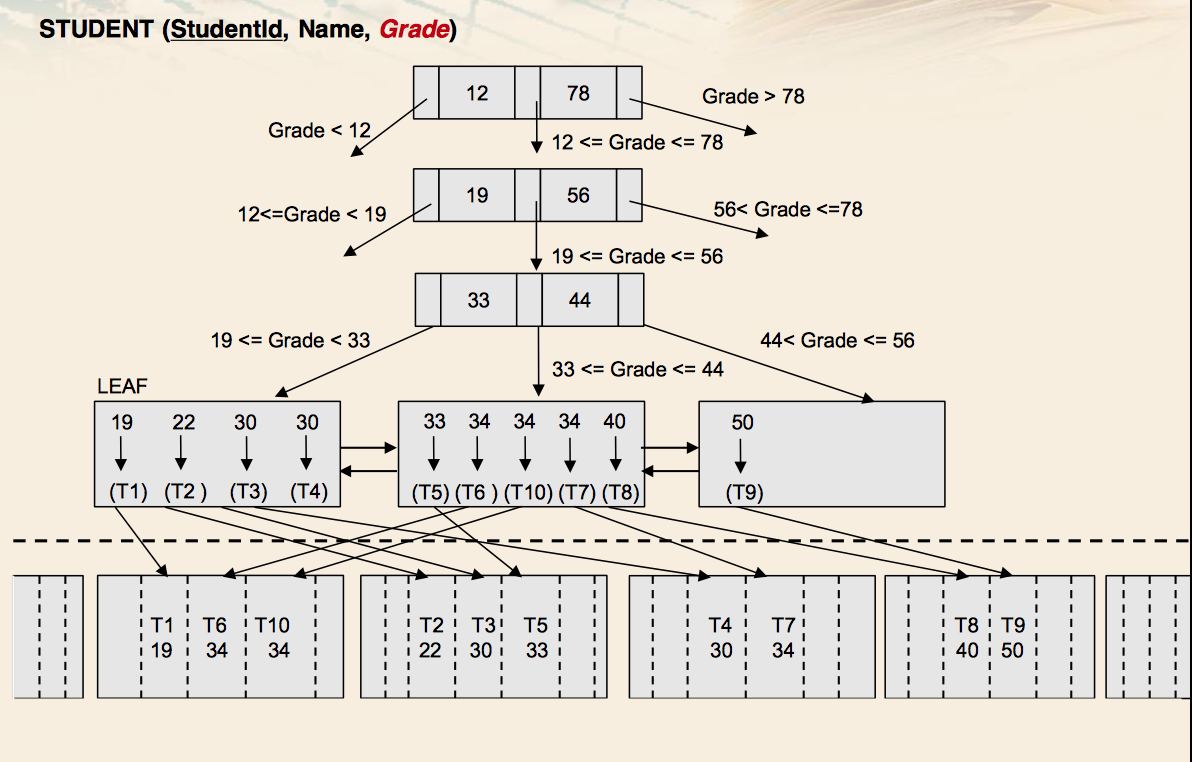
\includegraphics[width=\linewidth]{images/unclu.png}
    \caption{Unclustered}
    \label{fig:unclu}
  \end{minipage}\hfill
\end{figure}
There are two kind of B-Tree:
\begin{itemize}
  \item \textbf{B-Tree}: Data pages are reached only through key values by visiting the tree. [figure \ref{fig:b}]
  \item \textbf{$B^{+}$-Tree}: Provides link leaf allowing sequential access in the sort order. [figure \ref{fig:bplus}]
\end{itemize}
\begin{figure}[!hbpt]
  \centering
  \begin{minipage}{.45\textwidth}
    \centering
    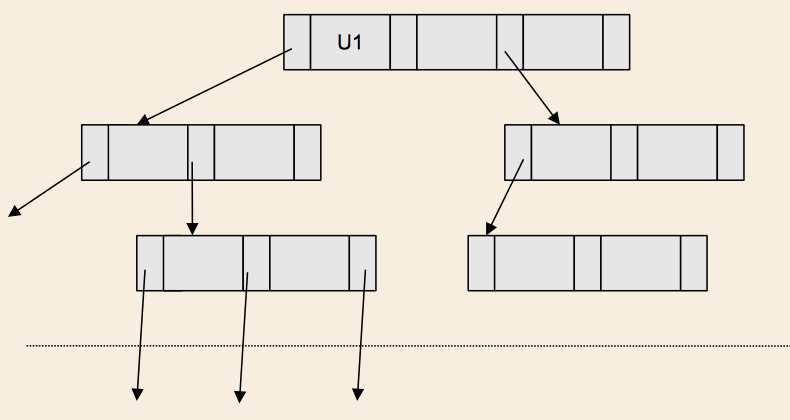
\includegraphics[width=\linewidth]{images/b.png}
    \caption{B-Tree}
    \label{fig:b}
  \end{minipage}\hfill
  \begin{minipage}{.45\textwidth}
    \centering
    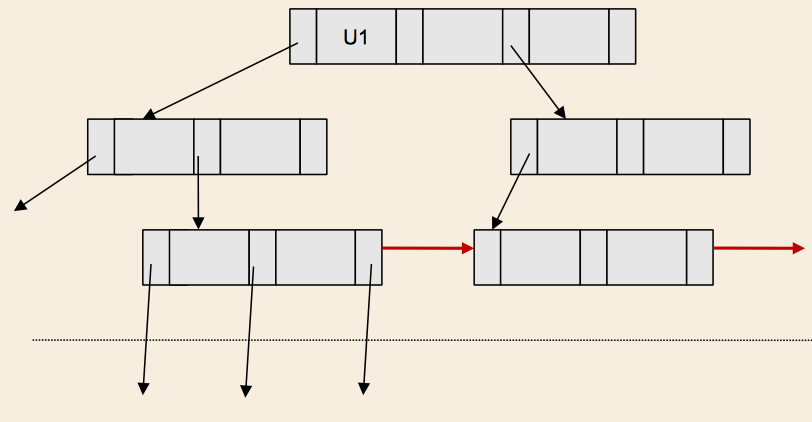
\includegraphics[width=\linewidth]{images/bplus.png}
    \caption{$B^{+}$-Tree}
    \label{fig:bplus}
  \end{minipage}\hfill
\end{figure}
the B stands for \textbf{Balanced} where leaves are all at the same distance from the root and the search time is the same indipendently by the value.\\
This structure have some:
\begin{itemize}
  \item \textbf{Advantages}:
  \begin{itemize}
    \item Very efficent for range queries.
    \item Appropriate for sequential scan in the order of the key field (always for clustered, not guarantee otherwise).
  \end{itemize}
  \item \textbf{Disadvantage}:
  \begin{itemize}
    \item Insertion may require a leaf or nodes split.
    \item Deletions may require merging uncrowded nodes and re-balancing.
  \end{itemize}
\end{itemize}

The \textbf{Hash} structure is another kind of weel-know structure is guarantees direct and efficent access to data based on the value of a key field (one or more attributes). Supposing to have B blocks in the hash structure the hash function is applied to the key value of a record and in return a values between 0 and b-1 which defines the position of the record, the idea is to not completly fill the blocks to allows new data insertion.
\begin{itemize}
  \item \textbf{Advantages}:
  \begin{itemize}
    \item Very efficent for queries with equality predicate on the key.
    \item No sorting of disk blocks is required.
  \end{itemize}
  \item \textbf{Disadvantage}:
  \begin{itemize}
    \item Inefficent for range queries.
    \item Collision may occur.
  \end{itemize}
\end{itemize}

The unclustered versione is similar to the hash index, the main difference is that the actual data is stored in a separate structure and the position of tuples is not constrained to a block.\\

The \textbf{bitmap index} is another structure that provides direct and efficient access to data based on the value of a key field, it's based on a bit matrix. The bit matrix references data rows by means of RIDs (Rows IDentifiers), the actual data is stored in a separate structure and the tuples position is not constrained.\\
The bit matrix has:
\begin{itemize}
  \item One column for each different value of the indexed attribute
  \item One row for each tuple.
\end{itemize}
the \textit{(i, j)} position has a 1 if the tuple \textit{i} as \textit{j} like attributes for the key field, 0 otherwise.
\begin{figure}[h!]
  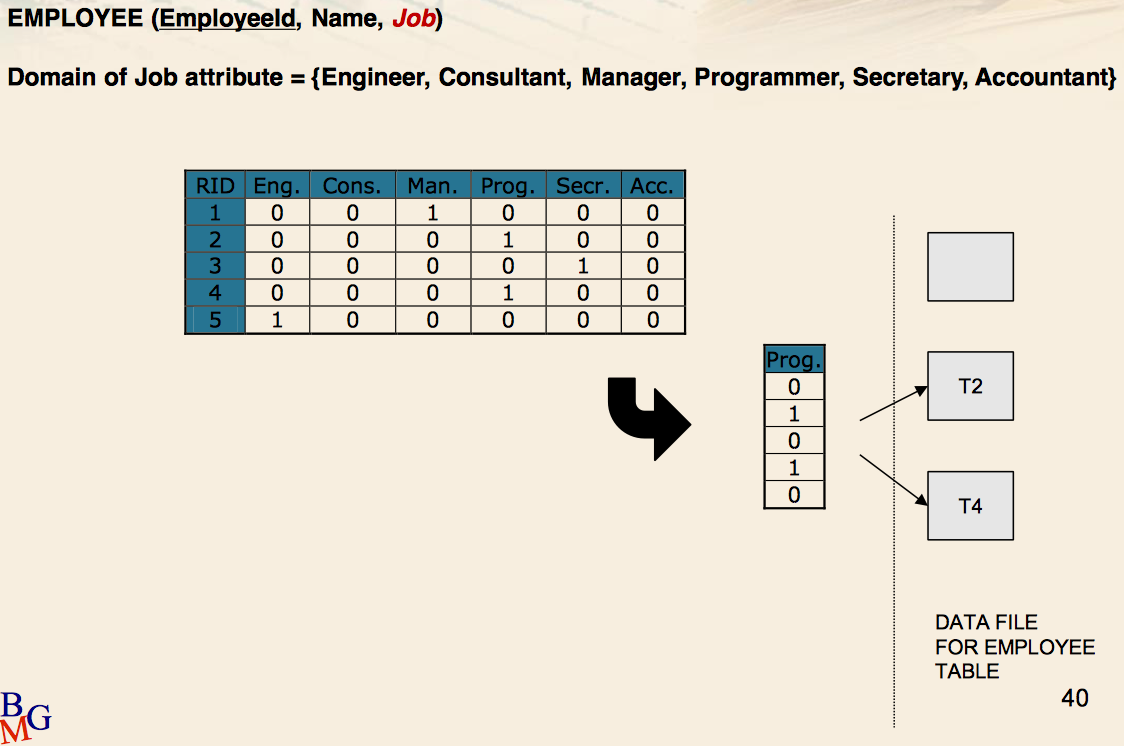
\includegraphics[width=\linewidth]{images/bitmapindex.png}
  \caption{Bitmap Index}
  \label{fig:bitmapindex}
\end{figure}
the main characteristics are:
\begin{itemize}
  \item \textbf{Advantages}:
  \begin{itemize}
    \item Very efficent for boolean expressions of predicates.
    \item Appropriate for attributes with limited domain cardinality.
  \end{itemize}
  \item \textbf{Disadvantage}:
  \begin{itemize}
    \item Not used for continuous attributes.
    \item Required space grows significantly with domain cardinality.
  \end{itemize}
\end{itemize}

\subsection{Query Optimization}
The query optimizer is part of the Optimizer and its job is selecting an efficient strategy for query execution, this block is really important. Another important task is to guarantees the data independence property, in fact, the form in which the SQL query is written does not affect the way in which it is implemented and a physical reorganization of data does not require rewriting SQL queries.\\
The query optimizer generates a \textbf{Query Execution Plan} to use the best strategies to run the query, it evaluates many different alternative, it use data statistics, use best-know strategies and it adapts automatically on data changes. The plan has more phases as you can see in figure \ref{fig:opt_plan}. The behaviour of each phase is:
\paragraph{Lexical, Synctactic and Semantic analysis}: check the SQL for Lexical errors (e.g., misspelled keywords), Syntactical errors in the SQL grammar and for Semantic erros not existing object called in the query (require data dictionary). The output of this block is an internal rappresentation of extended relational algebra because it can represent the order in which operators are applied (procedural) and there are a lot of theorems and properties.\\
\paragraph{Algebraic Optimization}: executing algebraic transformations is considered to be always beneficial, it should eliminate the difference among different formulations of the same query and is usually independet of the data distribution. The output of this phase is a "canonical" tree.\\
\paragraph{Cost Based Optimization}: This phase select the best execution plan evaluating the execution cost, it use a selection of:
\begin{itemize}
  \item Best access method for each table.
  \item Best algorithm for each relational operator among available alternatives.
\end{itemize}
the last step of this phase is the generation of the code implementing the best strategies, the output is the executable and all the dependencies used.\\
There are two types of execution modes:
\begin{itemize}
  \item \textbf{Compile and Go}: Compilation and immediate execution, no storage of query plan and no need of dependencies.
  \item \textbf{Compile and Store}: The plan is stored in the DB together with its dependencies, it's executed on demand and it need to be recompiled in data structure changes.
\end{itemize}

\begin{figure}[h!]
  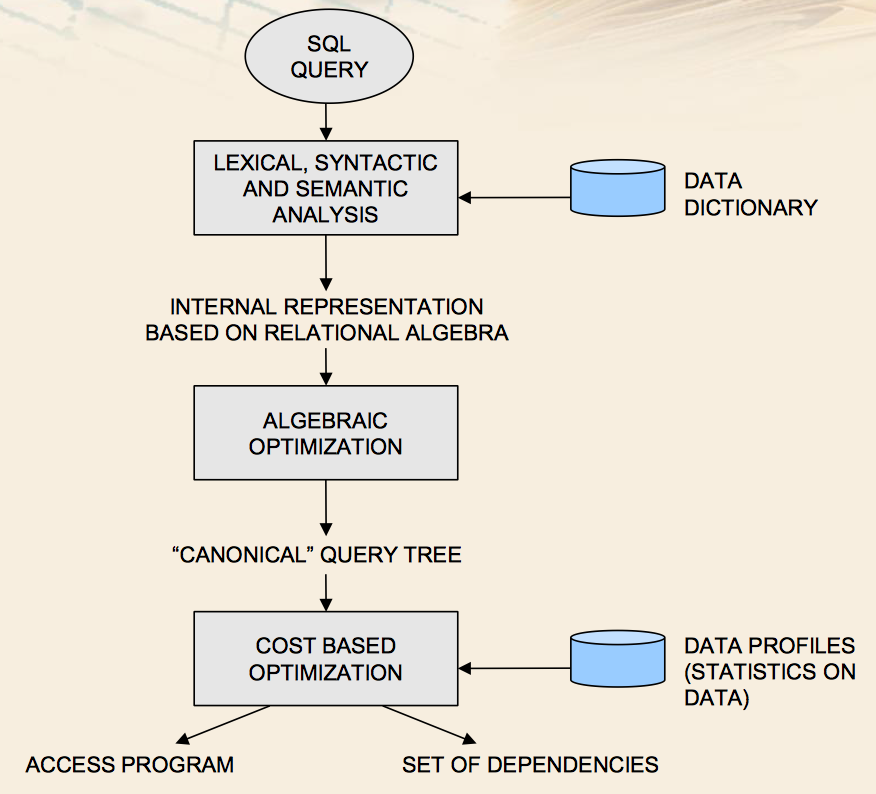
\includegraphics[width=\linewidth]{images/opt_plan.png}
  \caption{Optimization Execution Plan}
  \label{fig:opt_plan}
\end{figure}

The phase of \textbf{Algebraic Optimization} require a little more of analysis. The part is bbased on equivanlence trasformations, \textit{two relational expressions are equivalent if they both produce the same query result for any arbitrary database instance}. The main objective of this part is to \textbf{reduce the size of the intermediate result}.\\
There are some well-know transformation:
\begin{enumerate}
  \item \textbf{Atomization of selection}: Applying all attributes of selection one at the time or all together can provide different performance in case of indicies.
  \item \textbf{Cascading Projections}: It possibile to perform directly the final projection o doing more projections with different sub-set and you can obtain the same result.
  \item \textbf{Selection before join}: Anticipating the selection respect a join-operation can reduce the cardinality of the system reducing the number of operations for the join (is always used by the DBMS).
  \item \textbf{Join derivation from Cartesian Product}: Perform a cartesian product and then a selection over data get the same result as the join operation but more slowly.
  \item \textbf{Distributing selection respect union}: Is equivalent to select a sub-set and then merge it with another subset or merge the two set and then selecting it.
  \item \textbf{Distributing selection respect difference}: The formulas explain better: $\sigma_{F}(E_1 - E_2) = \sigma_{F}(E_1) - \sigma_{F}(E_2) = \sigma_{F}(E_1) - E_2 $.
  \item \textbf{Distributing projection respect union}: Projection of union of 2 table is equivalent to the union of 2 already projected table.
  \item \textbf{Other}: $\sigma_{F1 \vee F2}(E) = (\sigma_{F1}(E)) \cup (\sigma_{F2}(E))$
  \item \textbf{Other}: $\sigma_{F1 \wedge F2}(E) = (\sigma_{F1}(E)) \cap (\sigma_{F2}(E))$
  \item \textbf{Distributing join respect union}: Perform join of a table E with two merged table (E1 $\cup$ E2), is equivalent to join E with E1 and E2 separate and the merge it.
\end{enumerate}

The phase of \textbf{cost based optimization} is a little bit more complicated, it is based on:
\begin{itemize}
  \item \textbf{Data Profiles}: Statistical information describing data distribution for tables and intermediate relational expression.
  \item \textbf{Approximate cost}: Evaluating cost by looking at CPU, HDD and main memory usage and time.
\end{itemize}
The profilings of table save quantitavive information on the characteristics of tables and columns:
\begin{itemize}
  \item Cardinality of tuples.
  \item Size in bytes of tuples.
  \item Size in bytes of each attributes.
  \item Number of dinstinct values of each attribute.
  \item Min and max value of each attribute.
\end{itemize}
all this information are stored in the data dictionary that is periodically refreshed.\\

The access operators can perform different types of scans. The \textbf{sequential scan} execute sequential access to all tuples in a table (a.k.a Full Table Scan). The operation performed during a sequential scan:
\begin{itemize}
  \item Projection.
  \item Selection (Simple predicate).
  \item Sorting based on attribute list (memory sort or sort on disk).
  \item Insert, Update or Delete.
\end{itemize}
the predicate evaluation is fundamental to provide an efficent access to the data. The index access it may be exploit with all kind of structures, in case of simple equality predicate all structure are appropriate. Instead, for range predicate, the only appropriate one is the $B^{+}$-Tree. For predicates with limited selectivity full scan is better (if available bitmap could be used). In case of conjunction fo predicates the most selective one is evaluated first through the index, then the other. A possible optimization could be computing the intersection of bitmaps coming from available indices and then a table read for remaing predicates. In the disjunction the index access can be used only if all predicates have and usable index, otherwise FTS.\\

The \textbf{join} operation can be a critical operation for a relational DBMS, the connection between tables is based on values instead of pointer. There are several algorithms that can be used for the join:
\begin{itemize}
  \item \textbf{Nested Loop}: For each tuples of the outer table, the inner one is readed once. (BRUTE FROCE)
  \begin{itemize}
    \item Efficent when the inner tavle is small and fits in memory or when the join attribute in the inner table is indexed.
    \item Not cost symmertric. It depends on which table takes the role of inner.
  \end{itemize}
  \item \textbf{Merge Scan}: It sort the two tables on the join attribute and it start a parallel scan.
  \begin{itemize}
    \item Symmetric in terms of cost. Efficent for large and already-sorted tables.
    \item Requires sorting both table (already sorted or trough clustered index).
  \end{itemize}
  \item \textbf{Hash Join}: It applicate the same hash function to the join attrbute of both table. Tuples to be joined will fill the same bucket.
  \begin{itemize}
    \item Very fast join.
    \item Local sort and join is performed into each bucket.
  \end{itemize}
  \item \textbf{Bitmapped Join Index}: It precompute the join. The position (i,j) of the matrix is 1 if the tuple with RID j of A joins with tuple with RID i in table B and 0 otherwise.
  \begin{itemize}
    \item A data change need a recompute of table.
    \item Used in OLAP queries.
    \item It can exploit one or more bitmapped join indices (one for each pair of joined tables) and accessing the large central table is the last step.
  \end{itemize}
\end{itemize}

The \textbf{Group By} is one of the most important function of SQL and is performed in 2 different ways: The first one is the sort based, it sort the data on the group by attributes and the compute aggregate functions on groups; the hash based one instead it perform and hash function over data, sort the bucket just created and than compute the aggregate function.

\paragraph{Execution plan selection} is based on some data input, the data profiles (statistics over data) and the internal representation of the query tree, the output of this part is the "optimal" (it can't assure that it will be the best one) execution plan. This phase evaluate the cost of different alternatives for read tables and executing each relational operator exploting an approximate cost of execution.\\
The search is based on the following parameters:
\begin{itemize}
  \item Scan type of data (full scan, index).
  \item Execution order among operators.
  \item Type of operators implementation (different join methods).
  \item Sorting time (when).
\end{itemize}
The approach work on a tree of alternatives where each nodes represent a decision on a variable and the leaf one complete query execution plan. Of course the system select the cheapest one. The general formula is $C_{Total} = C_{I/O}*n_{I/O} + C_{CPU}*n_{CPU}$ where $n_{I/O}$ is the number of I/O operations and $n_{CPU}$ is the number of CPU operations.\\
The final plan is an approximation of the best solution. Th optimizer looks for a solution which is of the same order of magnitude of the "best" solution. In the \textbf{Compile and Go} execution mode the search is stopped when the time spend for the search is comparable to the time required to execute the current best plan. % 4_QueryOptimization finished

\subsection{Physical Design}
The physical distribution of the data in the system is fundamental for providing good performance. Taking in account the logical schema of the DB, the features of the selected DBMS and thw workload this block provides a physical schema of the databse (table organization, indices) and all necessary set up parameters for storage and configurations.\\
The possible physical file organization are:
\begin{itemize}
  \item Unordered (heap).
  \item Ordered (clustered).
  \item Hashing on hash-key.
  \item Clustering several relations.
\end{itemize}
The number of indicies is related to the structure type of the system. In case of clustered is possible to define only one index, instead, unclustered structures allow to define multiple different indices.\\
The workload distribution is different in case of a normal query or for an update. The first case involve:
\begin{itemize}
  \item Accessed tables.
  \item Visualized Attributes.
  \item Attributes involve in selections and joins.
  \item Selectivity of selections.
\end{itemize}
the update case instead:
\begin{itemize}
  \item Attributes and tables involved in selections.
  \item Selectivity of selections.
  \item Update type (Ins/Del/Up) and updated attributes.
\end{itemize}
The selection of the structure is important and it could be changed during the usage of the system for improvement (database tuning). Changes in the logical schema are allowed and they can or cannot preserve the BCNF (Boyce Code Normal Form). There isn't a general methodology the best solutions are trial and error, some general criteria and "common sense" heuristic.\\
Some general criteria could be:
\begin{itemize}
  \item Primary Key is usually exploited for selection and joins, indexing it could be useful.
  \item Adding new indices for most common query predicates. Evaluate the actual plan and verify the improvement if available.
  \item Never index small table, the entire table requires few disk reads.
  \item Never index attributes with low cardinality (e.g. gender). This is not true for data warehouses.
\end{itemize}
from the heuristics point of view there are severals "common sense" ideas:
\begin{itemize}
  \item For attributes involved in simple predicates of where clause equality:hash and range:$B^{+}$-Tree.
  \item Evaluated clustered improvement for slow queries.
  \item For where clauses involving many simple predicates use multi attributes index or appropriate key order.
  \item Maintenance cost.
  \item To improve joins use index on inner table in case of nested loop or $B^{+}$-Tree, for merge scan, on the join attribute.
  \item For group by hash index or $B^{+}$-Tree.
  \item Consider group by push down that anticipate the group respect to joins.
\end{itemize}
of course after all the changes a good choice could be update database statistics, for future improvements the database tuning could help. The last chance can be affecting optimizer decision, the main problem is the lost of data independence.

\subsection{Concurrency Control}
The workload of operational DBMS is measured in \textit{transaction per second} (banking and flight reservation are on 10-1000 tps). This block provide concurrent access to data maximizing the throughput and minimizing response time. The elementary operations are of course \textbf{READ r(x)} and \textbf{WRITE w(x)}. The block that manage the concurrency is called scheduler is in charge of deciding if and when read/write request can be satisfied.\\
The most common anomalies are:
\begin{itemize}
  \item \textbf{Lost Update}: It occur when a tr2 read a value that is already under operations by another tr. (figure \ref{fig:lost_update})
  \item \textbf{Dirty Read}: When a tr2 read the value of x in an intermediate state which never become permanent. (figure \ref{fig:dirty_read})
  \item \textbf{Inconsistent Read}: When a tr1 read multiples times x with different value each time. (figure \ref{fig:inco_read})
  \item \textbf{Ghost Update}: It occur when two transaction are working over multiple data at the same time performing read and write. (figure )
\end{itemize}

\begin{figure}[h!]
  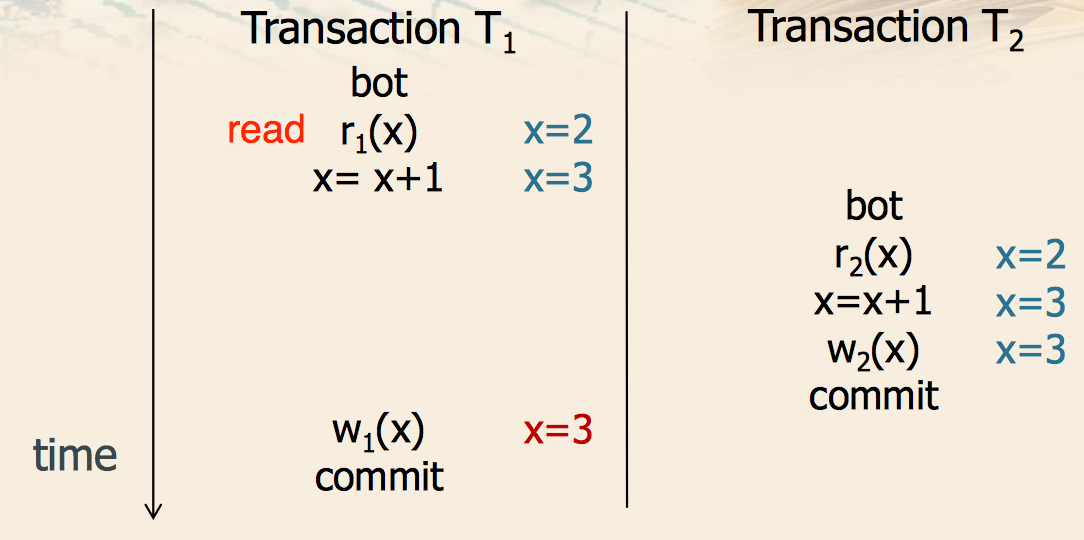
\includegraphics[width=\linewidth]{images/lost_update.png}
  \caption{Lost Update Behaviour}
  \label{fig:lost_update}
\end{figure}
\begin{figure}[h!]
  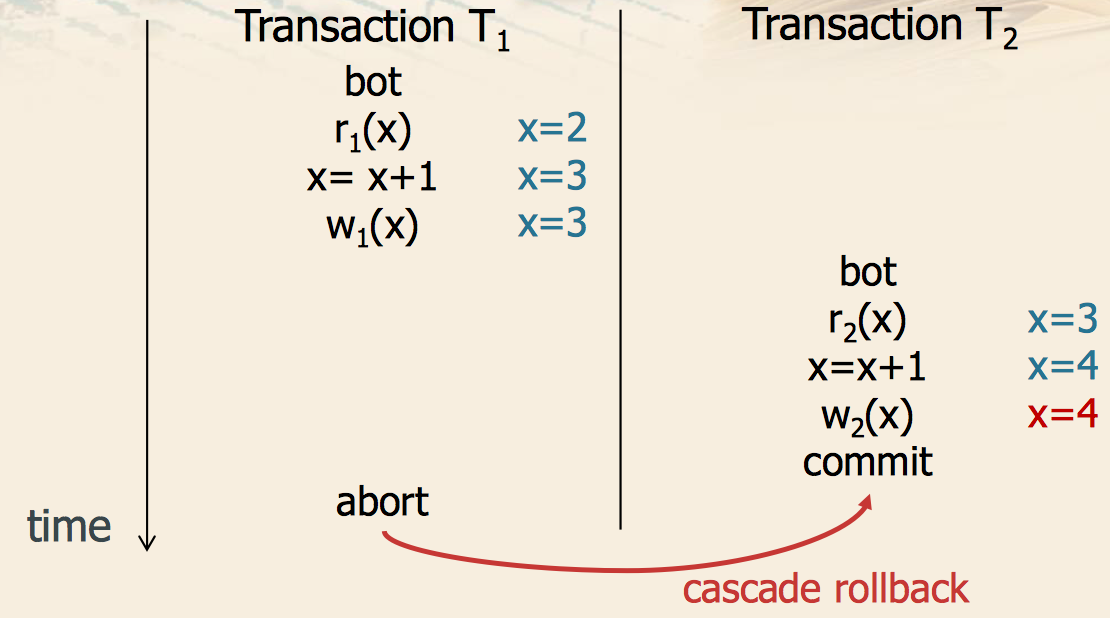
\includegraphics[width=\linewidth]{images/dirty_read.png}
  \caption{Dirty Read Behaviour}
  \label{fig:dirty_read}
\end{figure}
\begin{figure}[h!]
  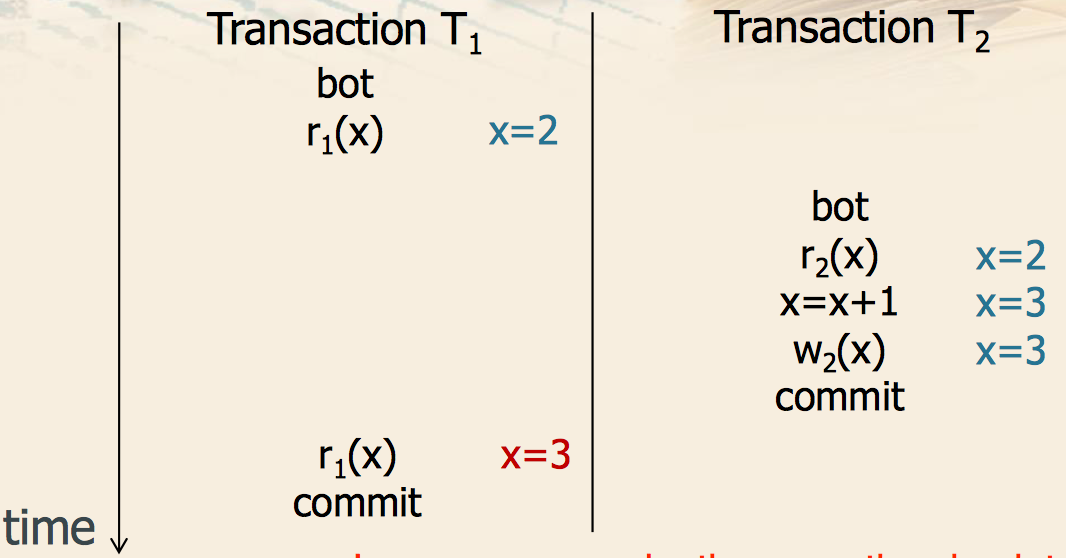
\includegraphics[width=\linewidth]{images/inco_read.png}
  \caption{Inconsistent Read Behaviour}
  \label{fig:inco_read}
\end{figure}
\begin{figure}[h!]
  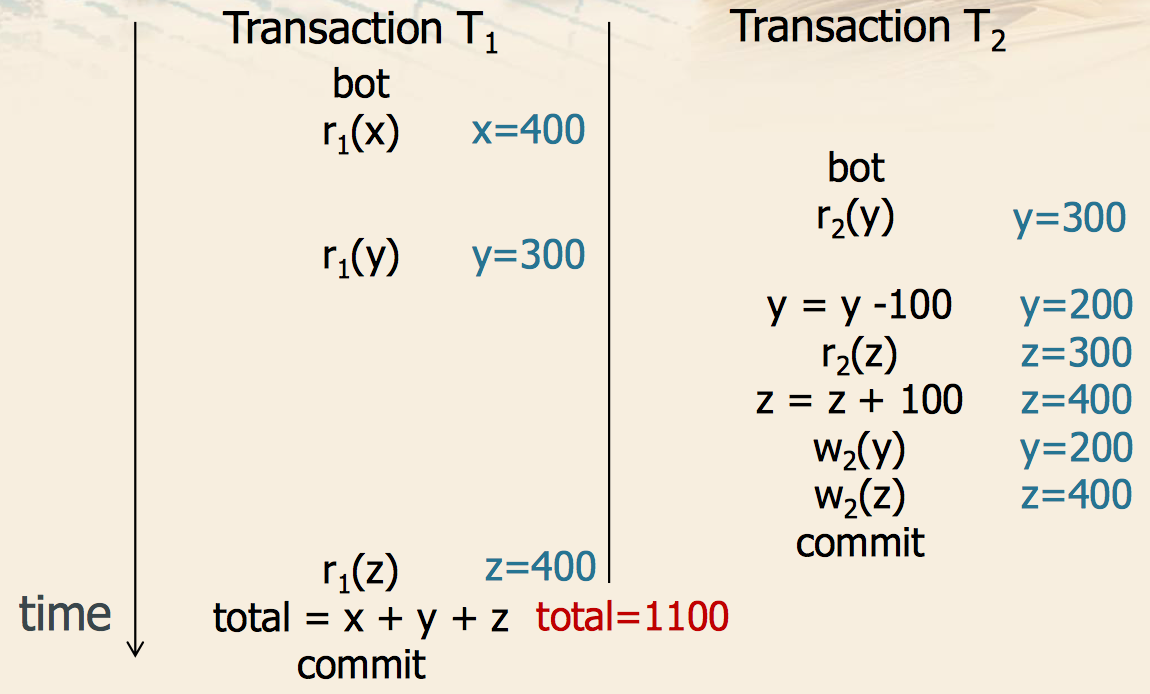
\includegraphics[width=\linewidth]{images/ghost_up.png}
  \caption{Ghost Update Behaviour}
  \label{fig:ghost_up}
\end{figure}

\paragraph{Theory of Control} a \textit{transaction} is a sequence of R/W operations with the same TID (\textit{Transaction Identifier}); the \textit{schedule} is a sequence of read/write operations presented by concurrent transaction. The scheduler is in charge of accepts or reject the requests to avoid anomalies without knowing the outcome (commit/abort) of it.\\
Commit projection is a simplifying hypothesis (the schedule only contains transaction performing commit), it avoid dirty read anomaly, it will be removed later.\\
In a \textbf{serial schedule}, the actions of each transaction appear in sequence, without interleaved actions. An arbitrary schedule $S_{i}$ is correct when it yields the same results as an arbitrary serial schedule $S_{j}$ of the same transactions. $S_{i}$ is serializable, is equivalent to an arbitrary serial schedule of the same transaction. There are different equivalence classes between two schedules:
\begin{itemize}
  \item View equivalence
  \item Conflict equivalence
  \item 2 phase locking
  \item Timestamp equivalence
\end{itemize}
each equivalence class find a set of acceptable schedules characterized by a different complexity.

\paragraph{View equivalence} there some definitions to be introduced:
\begin{itemize}
  \item \textbf{reads-from}: $r_{i}(x)$ reads-from $w_{j}(x)$ when:
  \begin{itemize}
    \item $w_{j}(x)$ precedes $r_{i}(x)$ and $i \neq j$
    \item There is no other $w_{k}(x)$ between them.
  \end{itemize}
  \item \textbf{final write}: is a final write if it is the last write of x appearing in the schedule.
\end{itemize}
with this solution two schedules are view equivalent if they have the same reads-from set or the same final write set.\\
This techniques is easy to be understand using an example. Using the flow in figure \refeq{fig:ex1}.
\begin{figure}[h!]
  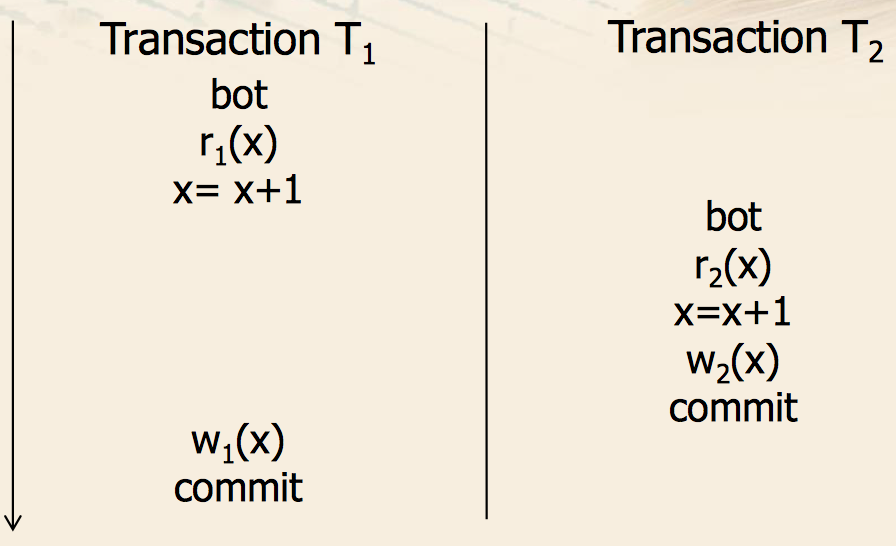
\includegraphics[width=\linewidth]{images/ex1.png}
  \caption{View Equivalence Example}
  \label{fig:ex1}
\end{figure}
The corrisponding schedule is: $S = r_{1}(x)r_{2}(x)w_{2}(x)w_{1}(x)$ is this schedule serializable?\\
There are only 2 possible serial schedules:
\begin{equation}
  \begin{gathered}
    S_{1} = r_{1}(x)w_{1}(x)r_{2}(x)w_{2}(x)\\
    S_{2} = r_{2}(x)w_{2}(x)r_{1}(x)w_{1}(x)
  \end{gathered}
\end{equation}
In both cases S is not view equivalent to any serial schedule, not serializable, should be rejected.\\
The analization of this problem is linear if the schedule is given, in case of an arbitrary schedule it become NP-complete. For this problem is better to use a less accurate, but faster techniques.

% Concurrency @ Pag. 30
\paragraph{Conflict equivalence}
Two actions are in conflict when both operate on the same object and at least one of them is a write. The conflict can be, RW, WR or WW. The conflict are equivalent if they have:
\begin{itemize}
  \item Same conflict set.
  \item Each conflict pair is in the same order in both schedules.
\end{itemize}
A schedule is conflict serializable (\textbf{CSR}) if it is equivalent to an arbitrary serial schedule of the same transaction.\\
Dectecting the conflict serializability it is possible to exploit the conflict graph:
\begin{itemize}
  \item Node: Each transaction.
  \item Edge i$\rightarrow$j: if is there at least a conflict between $T_{i}$ and $T_{j}$.
\end{itemize}
checking the cyclicity of a graph is linear in the size of the graph.

\paragraph{2 Phase Locking} a lock is block on a resource which may prevent access to others. The operations are:
\begin{itemize}
  \item \textbf{Lock}
  \begin{itemize}
    \item Read Lock (R-Lock)
    \item Write Lock (W-Lock)
  \end{itemize}
  \item \textbf{Unlock}
\end{itemize}
Each operation is preceded by a request of R/W-Lock and is followed by a request of unlock. Of course the R-Lock is shared among different transaction, the write lock instead is exclusive, not compatible with any other lock.\\
The scheduler becomes a lock manager it receives transaction requests and grants locks based on locks already granted and so on...\\
When the lock request id \textbf{granted}:
\begin{itemize}
  \item The resource is acquired by the requesting transaction.
  \item After the unlock, the resource, becomes again available.
\end{itemize}
When the lock is \textbf{not granted}:
\begin{itemize}
  \item The requesting transaction is put in a waiting state.
  \item The wait is terminated when the resources is unlocked and becomes available again.
\end{itemize}
All the information for grant or not the lock are stored in the \textbf{lock table} with the \textbf{conflict table} (figure \ref{fig:conflict}) used to manage lock conflicts.

\begin{figure}[h!]
  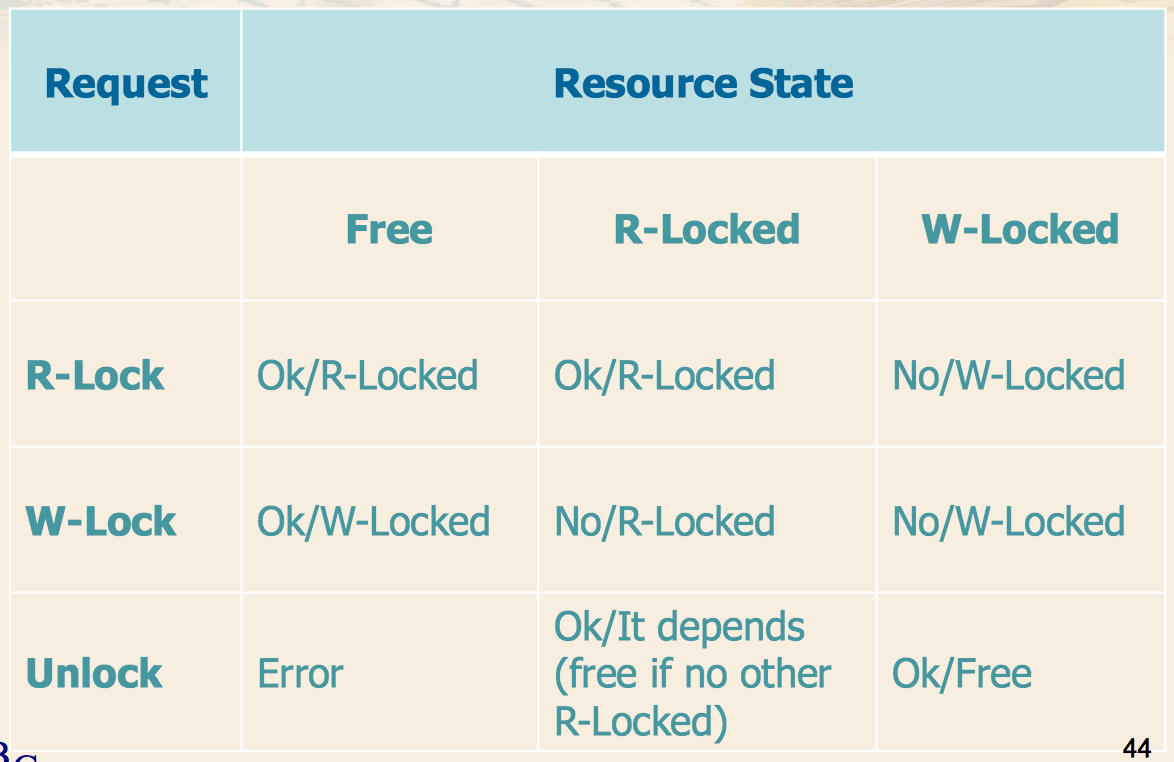
\includegraphics[width=\linewidth]{images/conflict.png}
  \caption{Conflict Table}
  \label{fig:conflict}
\end{figure}

The read locks are shared this is because the read not change the state of a data and multiple access can be exploited at the same time. A counter is used to count the number of R-Lock granted on a resources.\\
The lock manager, that coordinates the grant, exploit the lock table stored in main memory and, for each data object, use 2 bits to represent the 3 possible states (free, r-locked, w-locked) and a counter to count the number of waiting transaction. An example in figure \ref{fig:TwoPhaseEx}.

\begin{figure}[h!]
  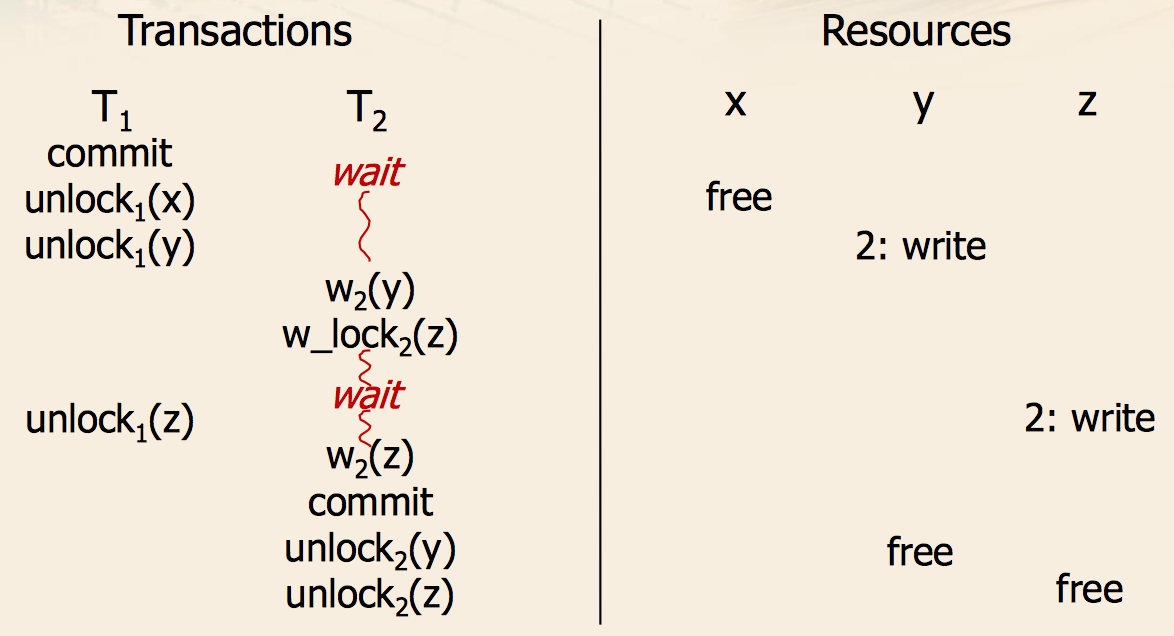
\includegraphics[width=\linewidth]{images/TwoPhaseEx.png}
  \caption{Conflict Table}
  \label{fig:TwoPhaseEx}
\end{figure}

There is also another version of the 2 phase locking the STRICT version. In this solution the unlock will be performed only at the end o the transaction and not when the resources is released; this difference guarantee to avoid the dirty read anomaly.\\
The procedure is really fast. If a transaction keep in wait over timeout the lock manager resume it and returns a NOT OK ERROR, the requesting transaction may perform a rollback o request again the same resources.

% Concurrency Control @ Pag. 57 = Hierarchical Locking
\paragraph{Hierarchical Locking} locks tables at different granularity levels:
\begin{itemize}
  \item Table
  \item Group of Tuples (fragment)
  \item Single Tuple
  \item Single Field in a Tuple
\end{itemize}
this is an extension of the traditional locking. It allows a transaction to request a lock at the appropriate level of the hierarchy and it is characterized by a large set of locking primitives.\\
The \textbf{Locking Primitives} are:
\begin{itemize}
  \item \textbf{Shared Lock (SL)}
  \item \textbf{eXclusive Lock (XL)}
  \item \textbf{Intention of Shared Lock (ISL)}: It shows the intention of shared locking on an object which is in a lower node in the hierarchy.
  \item \textbf{Intention of eXclusive Lock (IXL)}: Similar to ISL, but for exclusive lock.
  \item \textbf{Shared lock and Intetion of eXclusive Lock (SIXL)}: Shared lock of the current object and intention of exclusive lock for one or more objects in a descandant node.
\end{itemize}
The behavior is reported in figure \ref{fig:hierlock}.
\begin{figure}[h!]
  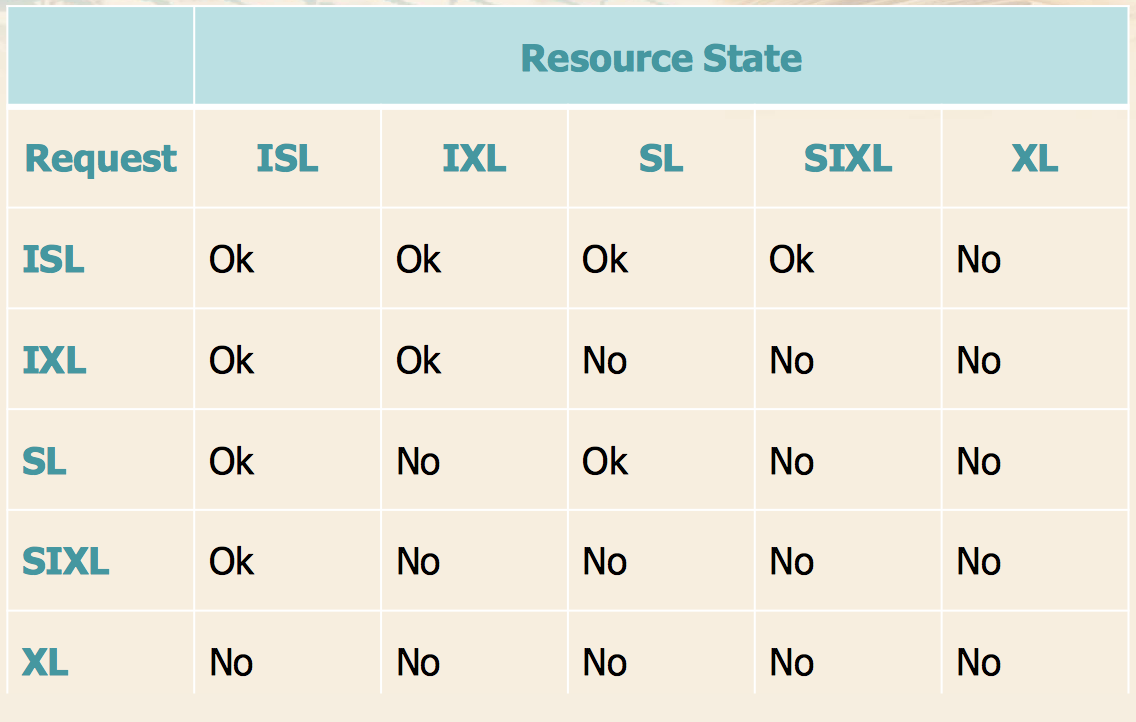
\includegraphics[width=\linewidth]{images/hierlock.png}
  \caption{Hierarchical Behavior}
  \label{fig:hierlock}
\end{figure}

The selection of lock granularity depends on the application type:
\begin{itemize}
  \item If it performs localized reads or updates of few objects (low lv - detailed ganularity).
  \item If it performs massive reads or updates (high lv - rough granularity).
\end{itemize}
the effect of lock granularity:
\begin{itemize}
  \item If it is too coarse, reduces concurrency.
  \item If it is too fine, it forces significant overhead on the lock manager.
\end{itemize}

The predicate locking addresses the ghost update of type b (insert) anomaly, for the 2PL a read operation is not in conflict with the insert of new tuple, they can't be locked in advance. The PredLock allows locking all data satisfying a given predicate.

There are several isolation level:
\begin{itemize}
  \item \textbf{SERIALIZABLE}:
  \begin{itemize}
    \item Highest
    \item PredLocking
  \end{itemize}
  \item \textbf{REPEATABLE READ}:
  \begin{itemize}
    \item Strict 2PL without PredLock
    \item Read existing obj can be correctly repeated
    \item No protection ghost update
  \end{itemize}
  \item \textbf{READ COMMITTED}:
  \begin{itemize}
    \item Not 2PL
    \item The read lock is released as soon as the object is read
    \item Reading intermediate states of a transaction is avoided (dirty reads)
  \end{itemize}
  \item \textbf{READ UNCOMMITTED}:
  \begin{itemize}
    \item Not 2PL
    \item Data reads without acquiring the lock
    \item Only allowed for read only transaction
  \end{itemize}
\end{itemize}

\textbf{Deadlocks} can be frequent, the solution for solving it are implementing \textbf{timeout} the transaction waits for a given time, after the expiration of TO it receives a negative answer and it performs rollback. The time length could be LONG and SHORT (can be overloads the system). Other solution can be performed Pessimistic 2PL that acquire all locks before the transactions start (not always feasible) or the timestamp that put in wait mode only younger transaction. The deadlocks detection is performed using the wait graph, it could be expensive to build and mantain.

\subsection{Reliability Management}
It is responsible of the atomicity and durability ACID properties, it implements the following transactional commands:
\begin{itemize}
  \item BEGIN transaction (B)
  \item COMMIT (C)
  \item ROLLBACK (A, for Abort)
\end{itemize}
it also provides recovery primitives WARM and COLD RESTART.\\
It manages the reliability of R/W requests by interacting with the buffer manager, it may generate new R/W requests for reliability purposes. It exploits the \textbf{log file} a persistent archive recording DBMS activity and is stored in a "stable" memory (not affected by failure, abstraction). It prepares data for performing recovery by means of the operations \textit{checkpoint} and \textit{dump}.\\
\paragraph{Log file} is a sequential file written in stable memory that records transaction activities in chronological order. The record can be related to a transaction or system, they are saved interleaved between different transaction.\\
The transaction log are written in this way:
\begin{itemize}
  \item BEGIN B(T)
  \item COMMIT C(T)
  \item ABORT A(T)
  \item INSERT I(T, O, AS)
  \item DELETE D(T, O, BS)
  \item UPDATE U(T, O, BS, AS)
\end{itemize}
where O represent the written object, AS is the After State (state of object O after modification) and BS is the Before State.\\

\textbf{Checkpoint} are periodically operation requested by the RM to the BM, it allows a faster recovery process. During the checkpoint, the DBMS writes data on disk for all completed transactions.\\
The flow of the checkpoint is:
\begin{enumerate}
  \item All the TIDs of all active transaction are recorded
  \begin{itemize}
    \item After the checkpoint start, no transaction can commit until the checkpoint ends.
  \end{itemize}
  \item The pages of concluded (C or A) transaction are synchronously written on disk.
  \begin{itemize}
    \item By means of the froce primitive.
  \end{itemize}
  \item A the end of step 2, a chekcpoint record is synchronously written on the log.
  \begin{itemize}
    \item Contains the set of active transactions.
    \item It is written by means of the focre primitive.
  \end{itemize}
\end{enumerate}

\textbf{Dump} is a complete copy of the database, typically performed when the system is offline, stored in stabel memory, may be incremental. At the end a dump record is written in the log.\\

The log is designed to allow recovery in presence of failure, WAL or Commit precedence. The WAL (Write Ahead Log, SYNC) the BS of data in a log record is written in stable memory vefore database data is written on disk, during recovery it will allows UNDO operation. The COMMIT PRECEDENCE (ASYNC) solution write the AS in a stable memory before commit, this will allows the execution of redo operations.\\

\paragraph{Recovery Management} there are two types of failures, the SYSTEM caused by software problem or power supply interruption that are causing losing in the main memoery content (buffer) but not on the disk. Or the MEDIA failure, caused by failure of devices managing secondary memory, this will lose the DB content on disk but not the log.\\
When a failure occurs the system is stopped, the type of recovery to be started depends on the failure type: SYS=WARM and MEDIA=COLD. When the recovery ends the system becomes again available to transactions.\\
The \textbf{WARM RESTART} is one of the solution for the recovery procedure:
\begin{itemize}
  \item All the transaction completed before the checkpoint not need a recovery action.
  \item The transaction which committed, but for which some write on disk are not already performed REDO is needed.
  \item Active transaction at the time of failure (not committed) UNDO is needed.
\end{itemize}
the checkpoint is not needed to enable recovery, it only provides faster restart, because, without it, the entire log until the last dump needs to be read. This solution reads backwards the log to detecs action which should be undo or redo, then star to read forward the log and perform all the actions.\\
The \textbf{COLD RESTART} is the second solution for recovery, it is performed when a portion of the database on disk get a failure. The main steps are:
\begin{enumerate}
  \item Access the last dump to restore the damaged portion of the DB on disk.
  \item Starting from the last dump record, read the log forward and redo all actions on the database and transaction commit/rollback.
  \item Perform a warm restart.
\end{enumerate}














\bibliographystyle{abbrv}
\bibliography{simple}

\end{document}
